\documentclass[hyperref={pdfpagelabels=false}]{beamer}
\usepackage{listings}
\usepackage{xcolor}

\definecolor{codegreen}{rgb}{0,0.6,0}
\definecolor{codegray}{rgb}{0.5,0.5,0.5}
\definecolor{codepurple}{rgb}{0.58,0,0.82}
\definecolor{backcolour}{rgb}{0.95,0.95,0.92}

\lstdefinestyle{mystyle}{
    backgroundcolor=\color{backcolour},   
    commentstyle=\color{codegreen},
    keywordstyle=\color{magenta},
    numberstyle=\tiny\color{codegray},
    stringstyle=\color{codepurple},
    basicstyle=\ttfamily\footnotesize,
    breakatwhitespace=false,         
    breaklines=true,                 
    captionpos=b,                    
    keepspaces=true,                 
    numbers=left,                    
    numbersep=5pt,                  
    showspaces=false,                
    showstringspaces=false,
    showtabs=false,                  
    tabsize=2
}

\lstset{style=mystyle}
% Contact information: 
%   Jorge M. Cruz-Duarte (jorge.cruz@tec.mx)
%   Nov. 29, 2019

\usepackage{lmodern, ragged2e, CJKutf8, booktabs, subfigure, graphicx, algorithm, algorithmicx, algpseudocode, amsmath, amssymb, amsthm, amsfonts, mathtools, multirow}
\usepackage[style=phys]{biblatex}
\addbibresource{bibliography.bib}
\renewcommand{\footnotesize}{\tiny}
\makeatletter
\@newctr{footnote}[page]
\makeatother
\usetheme{CambridgeUS}
\renewcommand{\raggedright}{\leftskip=0pt \rightskip=0pt plus 0cm}



\definecolor{TEC blue}{RGB}{0, 32, 159}
\newcommand{\hl}[1]{{\textcolor{TEC blue}{#1}}}

% Theme setup
\titlegraphic{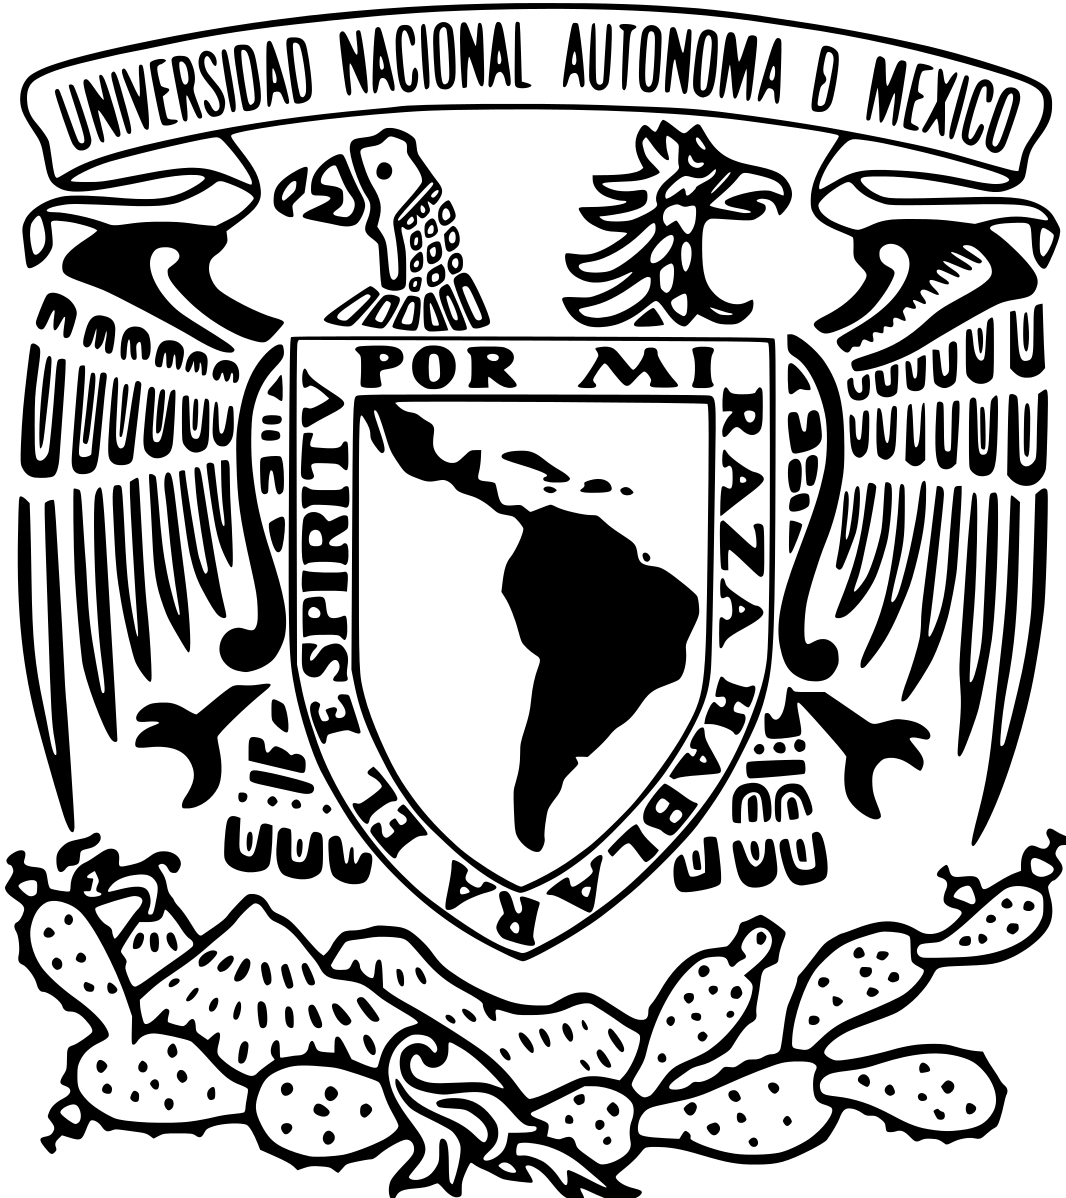
\includegraphics[scale=0.07]{Figures/logounam.png}}

% \makeatletter
\setbeamertemplate{headline}{%
\leavevmode%
  \hbox{%
    \begin{beamercolorbox}[wd=\paperwidth,ht=2.5ex,dp=1.125ex]{palette quaternary}%
    \insertsectionnavigationhorizontal{\paperwidth}{}{\hskip0pt plus1filll}
    \end{beamercolorbox}%
  }
}
\setbeamertemplate{footline}{\hspace*{2ex} \insertshortauthor \hfill \textcolor{TEC blue}{\insertshorttitle} \hfill \textbf{\insertframenumber{}} / \inserttotalframenumber \hspace*{2ex}}

\setbeamercolor{item projected}{bg=TEC blue}
\setbeamertemplate{enumerate items}[default]
\setbeamercolor*{enumerate item}{fg=TEC blue}

\setbeamertemplate{navigation symbols}{} 
% \setbeamertemplate{footline}[\insertshorttitle frame number]
\setbeamertemplate{bibliography item}[text]
\setbeamertemplate{theorems}[numbered]

\setbeamerfont{title}{series = \bfseries, parent = structure}
\setbeamerfont{frametitle}{series = \bfseries, parent = structure}
\setbeamerfont{headline}{series = \bfseries, size = \tiny, parent = structure}

\setbeamercolor{title}{fg = white, bg = TEC blue}
\setbeamercolor{frametitle}{fg = white, bg = TEC blue}
\setbeamercolor{structure}{fg = TEC blue}
\setbeamercolor{section in head/foot}{fg = black, bg = TEC blue!40}
\setbeamercolor{subsection in head/foot}{fg = black, bg = TEC blue!20}

\setbeamercolor{block title}{use=structure,fg=white,bg=structure.fg!75!black}
\setbeamercolor{block body}{parent=normal text,use=block title,bg=TEC blue!20} %block title.bg!10!bg}
\makeatletter
\def\th@mystyle{%
    \normalfont % body font
    \setbeamercolor{block title example}{bg=orange,fg=white}
    \setbeamercolor{block body example}{bg=orange!20,fg=black}
    \def\inserttheoremblockenv{exampleblock}
  }
\makeatother
\theoremstyle{mystyle}
\newtheorem*{remark}{Remark}

\usepackage{tikz}
\setbeamertemplate{background}{\tikz[overlay,remember picture]\node[opacity=0.05]at (current page.center){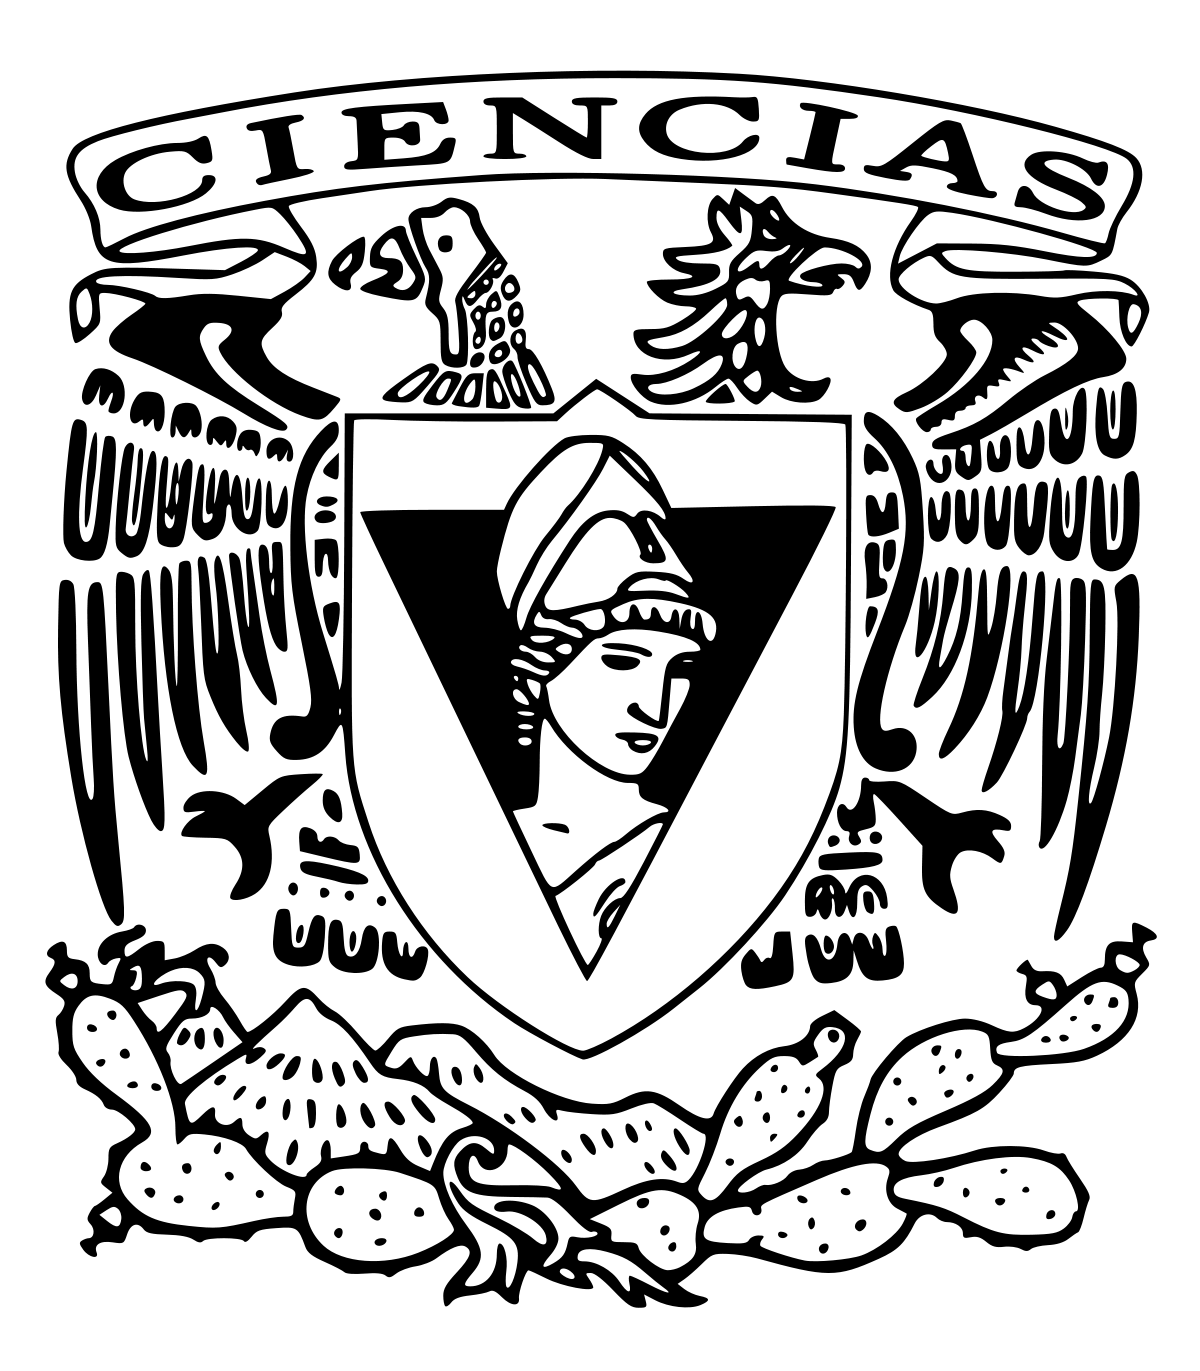
\includegraphics[width=6cm]{Figures/logociencias.png}};}


\newcommand{\maketitleandtoc}{%
{%
    \setbeamertemplate{headline}{}%
    \setbeamertemplate{footline}{}%
    \begin{frame}[noframenumbering]%
        \titlepage%
    \end{frame}%
    \begin{frame}[noframenumbering]%
        \frametitle{Contenido}%
        \tableofcontents%
    \end{frame}%
}}

\newcommand{\noheadfoot}[1]{%
    {%
        \setbeamertemplate{headline}{}%
        \setbeamertemplate{footline}{}%
        {#1}
    }
}

\title{Planetary Motion}  
\author[Facultad de Ciencias]{Miguel Ángel Sánchez Cortés} 
\institute{Facultad de Ciencias, UNAM} 
\date{\today}

\begin{document}

\maketitleandtoc

\section{Introduction}
\begin{frame}{The equations of motion}\justifying

One of the main contributions of Newton's Laws was the verification of Kepler's Laws of Planetary Motion.

\vspace{10pt}

\begin{figure}
        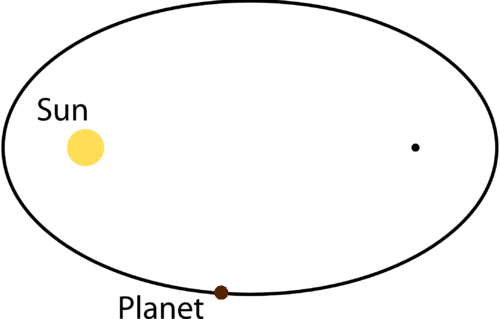
\includegraphics[width=0.4\linewidth]{Figures/kepler2.png}\\ \vspace{1cm}
    \end{figure}

\vspace{-15pt}

In this project we pretend to solve numerically this equations of motion with Newton's theory and analyze the results

\end{frame}
\begin{frame}{The equations of motion}

Suppose we have a planet of mass $m$ that orbits around another planet of mass $M \gg m$. 

\vspace{10pt}

Using polar coordinates, with $r$ the radial distance between the center of both planets and $\theta$ the angle between $r$ and the axis of symmetry, we obtain using Newton's Second Law and the Universal Gravitation Law that:


\begin{block}{The equations of motion}
\begin{equation}
m(r\ddot{\theta}+2\dot{r}\dot{\theta})=0 \quad \text{y} \quad m(\ddot{r}-r\dot{\theta}^{2})=-\frac{GMm}{r^{2}}
\end{equation}
\end{block}

The first of this equations is just the conservation of angular momentum and is equivalent to:

\begin{equation}
h=r^{2} \dot{\theta} = \text{constant}
\end{equation}

\end{frame}
\begin{frame}{The equations of motion}

Finally, substituting $(2)$ in $(1)$, we obtain the equations of planetary motion:

\begin{equation}
\ddot{r}=\frac{h^2}{r^3} - \frac{GM}{r^2} \quad \text{y} \quad \dot{\theta}=\frac{h}{r^2}
\end{equation}

that, without dimensions, are simply:
\begin{block}{Equations of planetary motion}
\begin{equation}
\ddot{r} = \frac{1}{r^3}-\frac{1}{r^2} \quad \text{y} \quad \dot{\theta}= \frac{1}{r^2}
\end{equation}
\end{block}
\vspace{10pt}

If we define $r_{p}=\dot{r}$, the equations become a system of 3 ODE:

\begin{equation}
  \dot{r_{p}} =\frac{1}{r^3}-\frac{1}{r^2} \quad \text{,} \quad 
  \dot{r} = r_{p} \quad \text{y} \quad 
  \dot{\theta} = \frac{1}{r^2}
\end{equation}
\end{frame}

\section{Development} 
\begin{frame}{Taylor's Method} 

We can solve the system of equations in $(5)$ using the second order Taylor Method. This method basically consists in solving an ODE in the following way:

\begin{equation}
\frac{dy}{dt}= f(t,y) \quad \text{with:} \quad y(a)= y_{ini}
\end{equation}

in an interval $[a,b]$ with constant spacing between the points given by $h=(b-a)/n$, where $n$ is the number of points, approximating the values of the function with a Taylor Series expansion:

\begin{block}{Taylor's Method}
\begin{equation}
y(t+h) \approx y(t) + y'(t)\cdot h + y''(t) \cdot \frac{h^2}{2}
\end{equation}
\end{block}






\end{frame}
\begin{frame}{Taylor's Method}

\begin{block}{For $r$ and $r_{p}$:}

\begin{equation}
\dot{r_{p}} =\frac{1}{r^3}-\frac{1}{r^2} \quad \text{y} \quad 
  \dot{r} = r_{p} \quad \text{with} \quad r_{p}(0)=0.2 \quad \text{and} \quad r(0)=1 
\end{equation}
\end{block}

with $h=0.001$ in the interval $[0,20]$, we approximate with the Taylor Series expansion:

\begin{align*}
r_{p}(t+h) &\approx r_{p}(t) + \dot{r_{p}}(t) \cdot h + \ddot{r_{p}}(t) \cdot \frac{h^2}{2} \\
r(t+h) &\approx r(t) + \dot{r}(t) \cdot h + \ddot{r}(t) \cdot \frac{h^2}{2}
\end{align*}

where the second derivatives are given by the ODE and are:

\begin{equation*}
\ddot{r_{p}} = \frac{-3\dot{r}}{r^4}+\frac{2\dot{r}}{r^3} \quad \text{y} \quad \ddot{r} = \dot{r_{p}}= \frac{1}{r^3}-\frac{1}{r^2}
\end{equation*}



    
\end{frame}

\begin{frame}{Taylor's Method}

\begin{block}{Also, for $\theta$:}

\begin{equation}
\dot{\theta} =\frac{1}{r^2} \quad \text{with} \quad \theta(0)=0
\end{equation}
\end{block}

with $h=0.001$ in the interval $[0,20]$, we approximate with the Taylor Series expansion:


 \begin{equation*}
\theta(t+h) \approx \theta(t) + \dot{\theta}(t) \cdot h + \ddot{\theta}(t) \cdot \frac{h^2}{2}
\end{equation*} 

where the second derivative is given by the ODE and is:

\begin{equation}
\ddot{\theta} = - \frac{2\dot{r}}{r^3}
\end{equation}

The next step is to implement this on Fortran.
\end{frame}



\begin{frame}{Plot for $\theta(t)$}

\begin{figure}
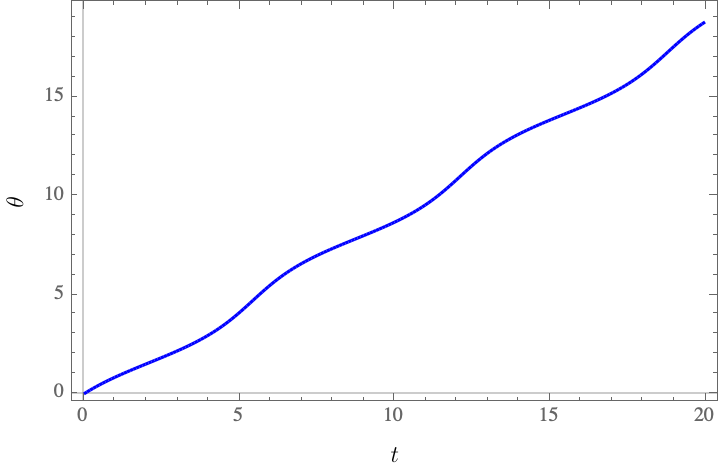
\includegraphics[width=0.8\linewidth]{Figures/thetavst.png}
\caption{Plot of $\theta \hspace{3pt} \text{vs} \hspace{3pt}  t$.}
\end{figure}
    
\end{frame}

\begin{frame}{In polar coordinates...}

\begin{figure}
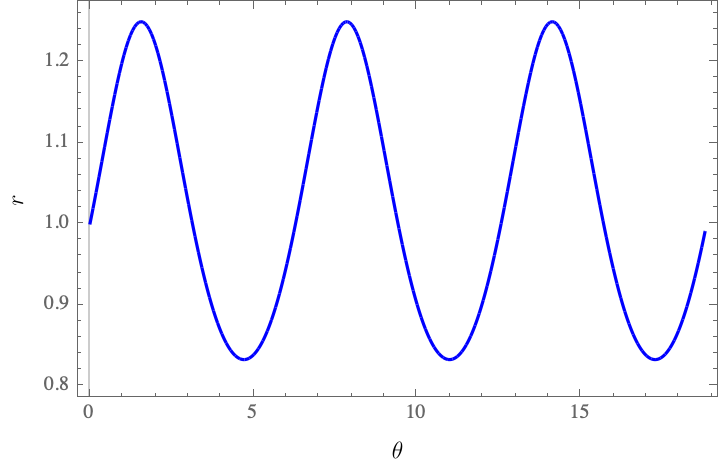
\includegraphics[width=0.8\linewidth]{Figures/rvstheta.png}
\caption{Plot of $r \hspace{3pt} \text{vs} \hspace{3pt}  \theta$.}
\end{figure}
    
\end{frame}

\begin{frame}{Finally, in cartesian coordinates...}

\begin{figure}
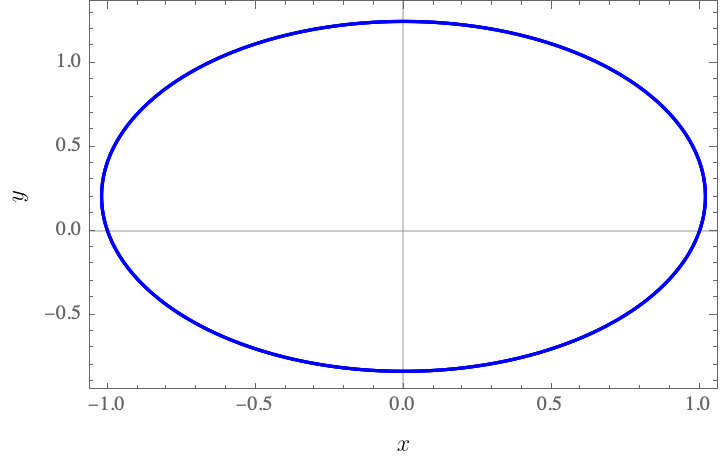
\includegraphics[width=0.8\linewidth]{Figures/trayectoria.png}
\caption{Plot of $y \hspace{3pt} \text{vs} \hspace{3pt}  x$.}
\end{figure}
    
\end{frame}

\section{Conclusion}

\begin{frame}{Conclusion}
\vspace{-10pt}

From the last plot, we can conclude that when we make the transformation from polar to cartesian coordinates:

\begin{equation}
x= r\cos(\theta) \quad \text{y} \quad y= r\sin(\theta)
\end{equation}

we see that the trajectory of the planet of mass $m$ is an \textbf{elliptic} trajectory.

This is a numeric proof of Kepler's 1st Law, who in 1609 wrote that:

\begin{block}{Kepler's 1st Law}

Every planet moves around the Sun describing an elliptic orbit where the Sun is at one of the foci of the ellipse.
\end{block}

    
\end{frame}


\noheadfoot{
\begin{frame}[noframenumbering]
\begin{minipage}[c]{0.3\linewidth}
\begin{flushright}
    \Large{
    \par \hl{!`Gracias!}
    \begin{CJK*}{UTF8}{gbsn}
    \par 谢谢!
    \par ありがとう!
    \end{CJK*}
    \par Thanks!
    \par Grazie!
    \par Merci!
    \par Mul\c{t}mesc!}
\end{flushright}
\end{minipage}\hspace{0.1cm}%
\begin{minipage}[c]{0.45\linewidth}
    \begin{flushleft}
        
\includegraphics[width=0.8\linewidth]{Figures/newton.png}
    \end{flushleft}
\end{minipage}%
\begin{flushright}
    \line(1,0){135}\\
    \textbf{Contact:}\\
    \hl{Miguel Ángel Sánchez Cortés}\\
    E-mail: \texttt{miguel.sanchezcortes@ciencias.unam.mx}\\
    \textit{Alumni}\\
    Facultad de Ciencias\\
    UNAM, Ciudad de México
\end{flushright}
\end{frame}
}

\end{document}

